\section{Conjoncture et politiques économiques} % (fold)
\label{prt:conjoncture_et_politiques_economiques}

Les différents organismes économiques, réalisent des prévisions de taux de croissance du PIB. Mais leurs prévisions divergent de part les modèles utilisés et 
les hypothèses réalisées.
L'approche macroéconomique de cette section, se base sur l'\emph{analyse de Keynes} 
et la \emph{synthèse néoclassique} ensuite opérée. 
On étudiera les \emph{modèles IS-LM} qui permettent donc de prévoir
les variations du PIB ainsi que l'impact au niveau du \emph{chômage} et de l'\emph{inflation}. 

L'économiste Kaldor propose d'analyser les phénomènes macro à l'aide du ``carré magique''.
Celui-ci est représenté à la Figure~\ref{fig:carre_magique} et on dira que la situation
économique d'un pays est jugée d'autant plus satisfaisante que la surface du quadrilatère
est proche de la situation idéale définie, dans ce cas-ci le carré en bleu.

\begin{figure}[h]
	\begin{center}
		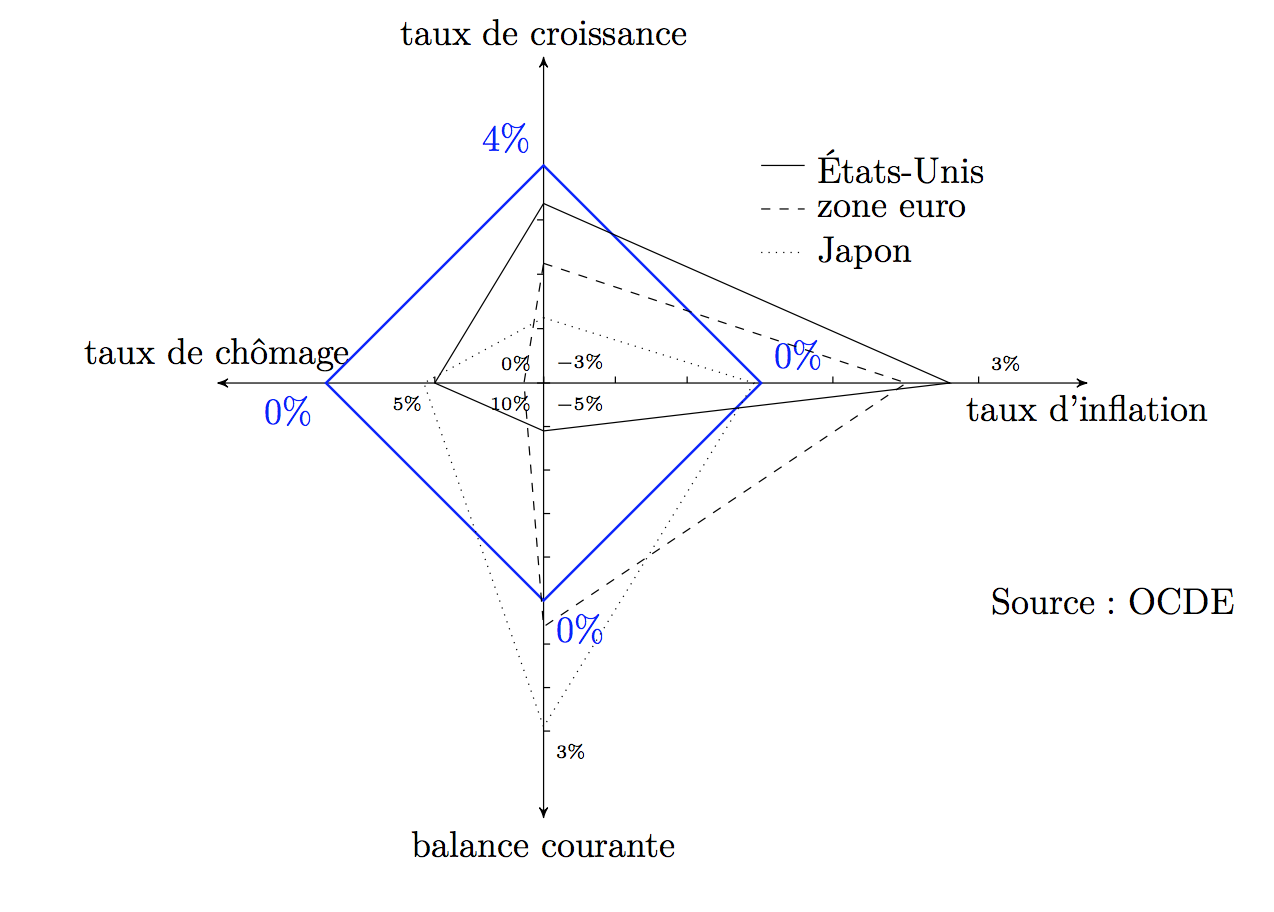
\includegraphics[scale=0.5]{./img/im2}
	\end{center}
	\caption{Carré magique : moyénné de 1996 à 2006}
  \label{fig:carre_magique}
\end{figure}

Les différents axes du \emph{carré magique} reprèsentent les objectifs de la politique macroéconomique. 
On s'intéressera dans ce chapitre aux trois premiers. 
On recueille différentes politiques économiques, chronologiquement discernables comme suit : 
\begin{itemize}[label=\ding{69}]
	\item \emph{Les trente glorieuses (45-73)} : une politique plus simple. 
  Une réponse parfaite à l'analyse keynésienne, en cas de récession et chômage élevé
	on instaurait des politques budgétaires et monétaires expansionistes (le contraire si chômage faible
  et inflation). On parle de politique de \textsc{Stop and Go}, la représentaiton économique 
  de ce phénomène s'appelle \emph{la courbe de Phillips}.
	\item \emph{À partir de soixante-dix} : on voit apparaître la \emph{stagflation}, c'est-à-dire un
  chômage croissant dans un environnement inflationniste. On retrouve pour cette période deux visions
  sur les fluctuations.
  \begin{enumerate}
    \item Selon les économistes \emph{néo-keynésiens}, l'État doit intervenir pour réguler le marché.
    \item Tandis que selon les \emph{nouveaux classiques}, l'État ne doit pas intervenir car les fluctuations
    sont des réponses naturelles du marché.
  \end{enumerate}
  \item \emph{Seconde partie des parties quatre-vingt} : la lutte contre l'inflation est le principal
  objectif des politiques. Celui-ci est atteint au moyen de politique budgétaire restrictive
  qui a entraîné des taux presque nuls et des soutiens des gouvernements moindres.
  \item Une poursuite de cette politique restrictive c'est vue causé par 3 éléments principaux : 
  \begin{enumerate}
  	\item Réunification allemande qui présentait un risque inflationniste de par le fort besoin de financement.
  	\item Mise en oeuvre de l'euro qui devait se présenter comme une monnaie forte.
  	\item Objectif majeur du déficit public imposé aux pays européens.
  \end{enumerate}
  \item Dans l'actualité on aurait pû se poser la question de la réalisation d'une politique expansioniste. C'est la crise de 2009 qui a poussé cette décision,
  en effet, pour protéger l'emploi. Cependant après une stabilisation, on a vu une déflation apparaître et la BCE à donc décidé de diminuer les taux pour 
  favoriser les invistissements et inciter les banques à réaliser des crédits.
\end{itemize}

Mais pourquoi la BCE ? Les états sont trop suceptibles de favoriser des injections dans un cadre démagogique, pré-élections. 

\subsection{Politique monétaire} % (fold)
\label{sub:politique_monetaire}

Kaldor stipule que l'illusion monétaire consistant à avoir une impression de hausse du pouvoir d'achat est grevé par l'inflation. Il n'est donc que purement 
démagogique de réaliser des politiques d'inflation avant des éléctions. De plus la courbe de Phillips stipulant qu'une hausse du pouvoir d'achat induit 
une baisse du chômage (Figure~\ref{fig:courbe_phillips}), est remise en cause par Friedmann qui stipule que les salariés anticipant l'inflation vont demander une hausse de
leur salaire afin de maintenir constant leur salaire nominal. Cette école classique est celle suivie par la BCE. Les principes de la BCE, se qualifient 
d'orthodoxie monétaire car ils consistent à établir une règle crédible et à s'y soumettre. 
\begin{figure}[h]
	\begin{center}
		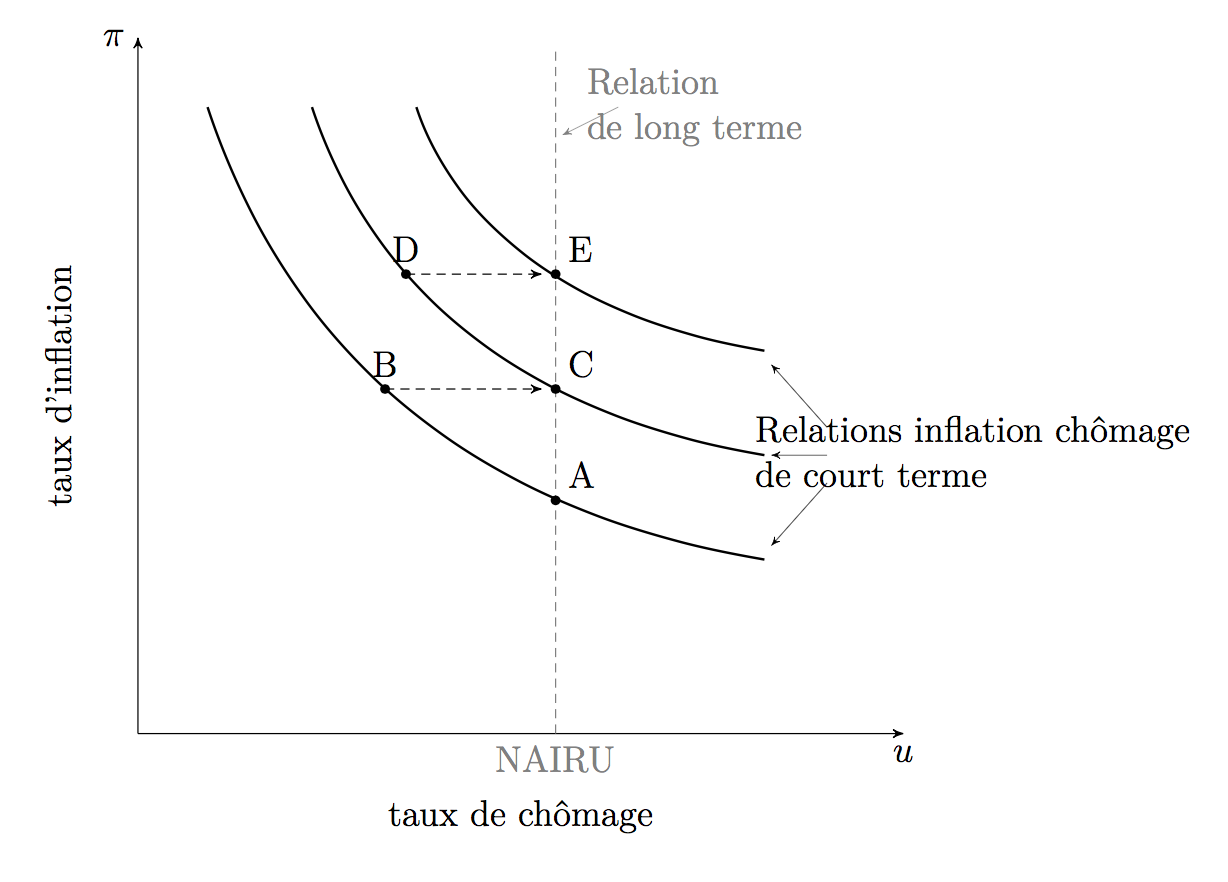
\includegraphics[scale=0.5]{./img/im3}
		
	\end{center}
	\caption{Courbe de Phillips}
  \label{fig:courbe_phillips}
\end{figure}
\newpage

Cependant ces règles sont parfois difficiles à assumer. Par exemple la stabilisation de l'inflation des années 80, a eû de fortes répercussions de croissance  en France, ainsi que l'implication d'une perte de l'avantage concurrentiel (dû au faible prix des produits français en relation aux autres).

On définit plus tard des politiques globales à l'Europe: 
\begin{enumerate}
	\item Taux d'inflation <1.5$\%$ de la moyenne des membres le plus performants.
	\item Devise devant rester au moins 2 ans dans le système monétaire.
	\item Intérêt moyen et long terme <$2\%$ des pays les moins inflationnistes.
	\item Dette <$60\%$ du PIB.
	\item Déficit public <$3\%$ du PIB.
	
\end{enumerate}

Un ensemble de contraintes, qui ne se voient fortement contrastées par les temps de crise ( dette France $\approx$ 100$\%$ PIB).

On présente 2 principes importants pour analyser la situation de la zone Euro. 

\textbf{Règle de Taylor}: 	\[
	\text{Taux d'intérêt}= f(\text{taux d'inflation-taux d'inflation cible},\text{taux de croissance-taux de croissance potentielle})
\]
\textbf{Mundell}: Seuls 2 des 3 objectifs suivants peuvent être atteints simultanéments: 
\begin{enumerate}
	\item Stabilité des changes.
	\item Liberté des mouvements des capitaux.
	\item Indépendance nationale des politiques monétaires. 
\end{enumerate}

La zone Euro à déjà obtenu la liberté de mouvement des capitaux, et ne s'impose pas de désir d'une stabilité de l'euro par rapport au dollar. Cependant pour le
dernier point, il est complexe de mener une politique commune dans une zone si diverse. Selon Mundell \emph{l'Europe n'est pas une zone monétaire optimale}.
Les conditions seraient réunies si : 
\begin{itemize}
	\item Faible degré d'asymétrie entre les chocs subis par les différents pays.
	\item Mobilité importante des facteurs de production, pour amortir les chocs. 
\end{itemize}
Ces conditions ne sont clairements pas réunies en Europe (par exemple la situation de la Grèce pendant la crise).
% subsection politique_monetaire (end)
\subsection{La politique budgétaire} % (fold)
\label{sub:la_politique_budgetaire}

\begin{tcolorbox}[title= Modèle IS-LM]
	
\end{tcolorbox}

% subsection la_politique_budgetaire (end)

\subsection{Le chômage} % (fold)
\label{sub:le_chomage}

Selon Keynes il est plus intéressant de favoriser la demande de travail que de baisser les salaires pour favoriser l'offre (en quantité).
Le chômage est moldé par les 2 forces suivantes : 
\begin{enumerate}
	\item \emph{Règle du côté court}, on ne peut obliger un agent à acheter un bien que s'il le désire au prix du marché. Donc l'entreprise produit que ce 
	qu'elle va vendre.
	\item Le chômage \emph{classique}, souffre aussi d'un double désequilibre. Offre inférieure à la demande sur le marché des biens, (réduction de l'offre
	en raison des coûts de production élevés). Offre supérieure à la demande sur le marché des biens (demande de travail des firmes réduite de part 
	le coût de la main d'oeuvre).
\end{enumerate}

La persistance du chômage a un lien direct avec le salaire. pour analyser ce dernier on analyse 2 théories récentes : 
\begin{itemize}
	\item \emph{Salaire d'efficience}, c'est un salaire supérieur au salaire moyen pour inciter le salarié à travailler.
	\item \emph{Négociations salariales}, les syndicats éssaient de faire augmenter le salaire et les conditions de travail, le revers de la négociation 
	est la création d'un chômage involontaire.
\end{itemize}

% subsection le_chomage (end)

% section conjoncture_et_politiques_economiques (end)